\documentclass[b5paper]{article}

\usepackage[english]{babel}
\usepackage{verbatim,ifthen,xspace,blindtext,datetime}
\usepackage{hyperref}
\usepackage{todonotes}

\RequirePackage{ifxetex}
\ifxetex
  \usepackage{fontspec}
  \setmainfont[Ligatures=TeX,Scale=MatchUppercase]{TimesNewRomanPSMT}
  \setsansfont[Ligatures=TeX,Scale=MatchUppercase]{Arial} 
\else
  \usepackage[utf8]{inputenc}
  \usepackage[T1]{fontenc}
  \usepackage{mathptmx}
\fi

%
\usepackage[%
  department=compute,    % select your department
  %bgcolor=dtulightgreen, % the colour of the tiles
  licolor=dtured         % the colour of the line
  ]{dtucover}
%
% We start by drawing the cover page and putting test onto it
\AtBeginDocument{
  \dtucoverThreeTiles % make the title page background
  \dtucoverTitleText %
    [Implementation of concurrent assertions in Chisel] % This is the subtitle
    {Assertions with time} % This is the title
    {Report} % This is the report type
    {Victor Alexander Hansen \\ Niels Frederik Flemming Holm Frandsen \\ DTU Compute \\ \monthname{} \the\year} % This is the author information
  \clearpage
}
% ... and at the end, we need the back cover
\AtEndDocument{
  \clearpage
  \dtucoverBackMatter%
    [                                     Gadenavn 00 \\ Evt. Post Box 000 \\ 0000 Bynavn \\ Tlf. 00000000 \\ Fax 00000000 \\~ \\ www.institut.dtu.dk]%
    [\blindtext]%
    [\textbf{Partner Corporation} \\ ~ \\ Gadenavn 11 \\ Evt. Post Box 111 \\ 1111 Bynavn \\ Tlf. 11111111 \\ Fax 11111111 \\~ \\ www.partner.dtu.dk ]%
}

\begin{document}

\section{Introduction}

This paper describes the path the authours have gone to be able to create an assertion-function which includes timing in chisel.

\section{Assertions in software and HDL}

We will in this section be relating to the simple scenario where we have a signals "a" and "b". There is then a criteria where "b" should be true a certain amount of clock cycles after "a" has gone high.
\smallskip
Concerning assertions in software, we look into Java assertions, as Scala runs on the JVM.
From the \href{https://docs.oracle.com/javase/7/docs/technotes/guides/language/assert.html}{\color{blue}Oracle Java SE Documentation} \texttt{assert} is a statement that enables boolean testing of assumptions in a program. If the boolean value returns true, the program proceeds as normal, if it returns false it throws an \texttt{AssertionError}.\\
Java has a concurrent utility, which allows the developer to use the \texttt{Waiter}
% https://jodah.net/concurrentunit/javadoc/}
class, to perform multi-thread assertions and wait for operations in threads to finish. If any of the assertions fails, the entire test fails, regardless of which thread failed. From the GitHub repository \href{https://github.com/jhalterman/concurrentunit}{\color{blue}concurrentunit} by jhalterman, toolkit is explained in details along with examples. Essentially, when a new thread is used for an assertion, \texttt{await} can be called, as in the example below, with or without an integer to specify the max delay for the htread to wait.

The main takeaway from concurrent assertions in Java, is that the developer in the test code deliberately creates multiple threads for the assertions to run concurrently with the code.\\
\smallskip

Concerning HDL, we look into SystemVerilog, more specifically, the keyword \texttt{Property} used in combination with an immediate assertion.

In SystemVerilog an assertion with
\href{https://www.chipverify.com/systemverilog/systemverilog-assertions-time-delay}{\color{blue}timing} can be done by using the keyword \texttt{sequence} and it's corresponding keyword \texttt{endsequence} with the statement \texttt{@(posedge clk) a \#\#x b;} inbetween these keywords, where x is the amount of clock cycles later "b" has to be high at. This now checks every rising edge of a clock cycle if "a" is high and if "b" is high a certain amount(x) of clock cycles later. You can then use the immediate assertion function \texttt{assert} to test if this statement is true. This will then give you an error if "b" is not high at exactly the specified amount of clock cycles later.
This solution has a flaw in the fact that "b" has to be high at the exactly at the specified amount of clock cycles later. So if "b" is high before that point, but then goes low again before you reach the specified clock cycle interval, then the assertion will still give you an error. This is a problem, if you want to check if the signal "b" goes high within a certain time frame. This can perhaps be altered so by stepping the number after the two hashtags in the earlier mentioned code with a loop.

\section{Specifications}
Assert\_never: a window in which an event is not expected\\
Assert\_always: a window where an event is expected\\
Assert\_eventually: a window bounding a check for a liveness property violation\\
Assert\_eventually\_always: like the beforementioned assertion, except that once the property occurs, it must remain valid until the ending event-trigger or the end of the simulation occurs\\
Assert\_one\_hot: checks for one hot encoding violationsassert


\section{Counting clockcycles}
The clock in Chisel is implicit. This implicit clock is driven by the testdriver in Chisel which uses the smallest time step, which is one cycle of the implicit clock.

Timing in Chisel can be achieved through counting clock ticks. Ticks are signals which are high for a single cycle. To determine when a tick must occur, one must divide the clock frequency of the design with the desired tick frequency. This way, we are not as much counting clock cycles, as we are determining the amount of clock cycles to pass before a certain event occurs.

This is pretty good, https://github.com/ucb-bar/chisel-testers2/issues/14

So apparently, \texttt{withClock()} and \texttt{Clock()} are things that just might be useful. 

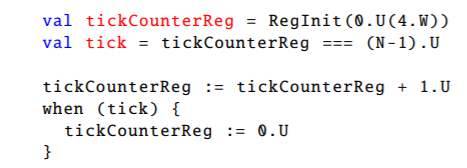
\includegraphics{Tickcount.PNG}

\section{Operating the clock}


\section{Test example}


\end{document}